\chapter{Strategie}

\section{Ziele}

\section{Wirkung}

\section{Zielgruppe}

\chapter{Ideenbeschreibung}
Momentan fährt der Roboter nur auf eine Position mit dem Behälter darauf. Diese fahrt wird durch die Software des Logistiksystems mitsamt des Roboters gesteuert. Neu soll die Software dieses Herstellers so erweitert werden (Siehe \ref{sec:roboterSWAnpassung}), dass der Roboter einen vordefinierten Pfad abfährt mit einem Spezifischen RFID Lesebehälter/Suchbehälter (Siehe \ref{sec:behaelterMitRFID}) und dabei noch Aktionen ausführt, wie einen Behälter für Kurze Zeit auszutauschen.
Würde nun ein Buch, welches von einer Bibliothek oder einem anderen Kunden bestellt wurde, nicht im Entsprechenden Behälter zu finden sein, soll neu der Spezielle RFID Lese-/Suchbehälter in das Hochregallager geschickt werden.


Dabei gibt es 2 Unterschiedliche Suchvorkehrungen. Als erstes würde der Roboter mit dem Lese-/Suchbehälter in alle Gassen geschickt, wo Roboter durch jede Reihe nacheinander fährt. Dabei wird jeweils vom Lese-/Suchbehälter der Vordere Behälter nach dem fehlenden Exemplar abgesucht. So kann in einer Kurzer Zeit ca. 50\% des Lagers nach dem deplatzierten Exemplar abgesucht werden. Würde nach diesem Suchvorgang die Lokalisation des Exemplares nicht erfolgreich abgeschlossen werden, würde in der Nacht die 2 Suchfunktion starten, bei welcher der Lese-/Suchbehälter im Hochregallager in der Höhe jeden dritten Platz eines äusseren bereits abgesuchten Behälters für eine kurze Zeit tauscht. Während der Lese-/Suchbehälter am äusseren Platzt ist sucht er im hinteren Behälter nach dem Exemplar sowie in den zu dem abgesuchten behälter direkt darüber sowie darunter befindlichen Behälter.

\section{Anpassungen Lagerverwaltungssoftware}
\label{sec:roboterSWAnpassung}
Für die Software der Lagerverwaltung soll die Herstellerfirma dieser Softer diese um eine Schnittelle erweitern, welche es ermöglicht über das Netzwerk neue Fahrpositionsdaten mitzuteilen, zu welchen der Roboter anschliessend fährt. Es soll dabei möglich sein dem Roboter zu sagen, ob er einen Behälter Tauschen soll oder nur an deren Position zu fahren. Zudem soll die momentane Position des Roboters über diese Schnittelle abgefragt werden können. 

\section{Behälter mit RFID Ausrüstung}
\label{sec:behaelterMitRFID}
Die heutige RFID HF technologie, welche bereits in der Speicherbibliothek zum Einsatzt kommt ist auf ca. 1m Distanz beschränkt. Dies bedeutet, dass es nicht möglich ist alle Tags direkt vom Roboter aus zu Lesen. Um alle Behälter auslesen zu können muss also der Behälter die Position eines anderen Behälters einnehmen um den Hinteren Behälter lesen zu können. Da es jedoch enorm Zeitintensiv ist, jede vordere Kiste mit dem Lese-/Suchbehälter auszutauschen, sollen multiple Antennen zum einsatzt kommen. Diese sollen so ausgerichtet werden, dass nicht nur der Hintere behälter sondern auch deren Nachbarn ausgelesen werden können.
Die Antennen sollen gemäss Abbildung \ref{fig:antennenPositionen} ausgerichtet werden.

\begin{figure}
	\centering
	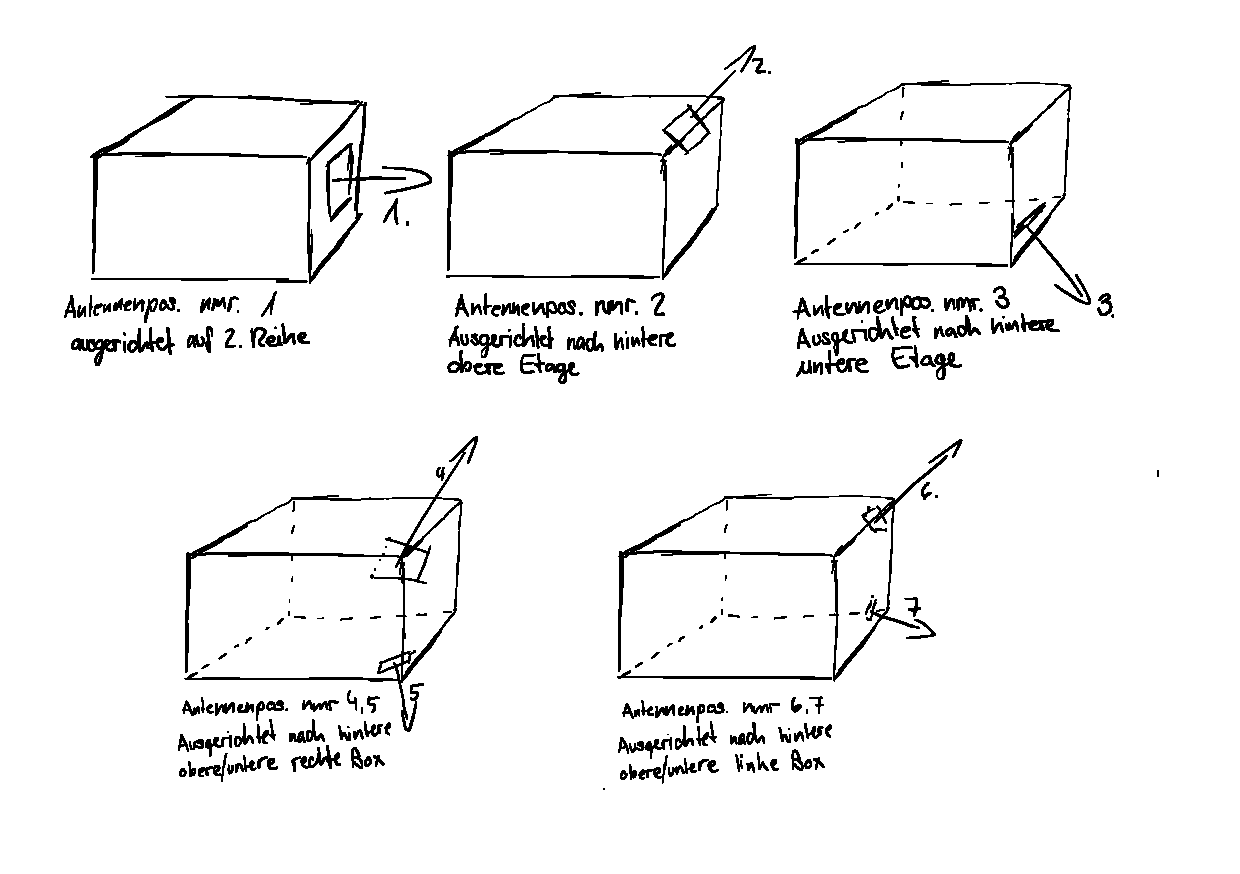
\includegraphics[keepaspectratio, width=1\textwidth]{antennen_auf_behaelter}
	\caption{Alle Antennenpositionen in einer Box für die Rechte Seite}
	\label{fig:antennenPositionen}
\end{figure}


\chapter{Zeitplan}

\chapter{Finanzierungsplan}

\chapter{Dokumentation und Evaluation}